% slides-exemplo-beamer
%
% Sáb Out  1 19:47:43 BRT 2011
%\pdfminorversion=7 
\documentclass[table, usenames, svgnames, xcolor=dvipsnames]{beamer}
\usepackage{beamerthemeshadow}
\usepackage[absolute,overlay]{textpos}
\usepackage{array}
\usepackage[brazil]{babel}  % adequacao para o portugues Brasil
\usepackage[utf8]{inputenc} % Determina a codificacao utiizada
                            % (conversão automática dos acentos)
\usepackage{makeidx}        % Cria o indice 
%\usepackage{movie15}
%\usepackage{flashmovie}
\usepackage{multimedia}
\usepackage{hyperref}     % Controla a formacao do indice
\usepackage{lastpage}       % Usado pela Ficha catalografica
\usepackage{indentfirst}    % Indenta o primeiro paragrafo de cada secao.
\usepackage{xcolor}          % Controle das cores
\usepackage{graphicx}       % Inclusao de graficos
\usepackage{subfig}
\usepackage{amsmath}        % pacote matemático
\usepackage{amssymb}
\usepackage{amsthm}
\usepackage{hhline}
\usepackage{tikz}
\usetikzlibrary{calc}
\usepackage{multirow}
\usepackage{bigstrut}
\usepackage{algpseudocode}

\usepackage{setspace}
\usepackage{caption}
\captionsetup[table]{singlelinecheck=false}
\captionsetup[figure]{slc=off}
\captionsetup{font=singlespacing}
\captionsetup{tableposition=top}

%\usepackage{subfigure}
%\usepackage{multicol}
%\usepackage{colortbl}

% ---------------------------------------------------------------------------- %
% Definições beamer
% ---------------------------------------------------------------------------- %
\usetheme{Copenhagen}
%\usetheme{Luebeck}
\usecolortheme{rose}

% Algumas definições para o layout
\setbeamerfont{frametitle}{size=\normalsize}
\setbeamerfont{title}{size=\normalsize}
%\setbeamertemplate{subsection in toc}
%\defbeamertemplate{subsubsection in toc}[subsubsections numbered]
\beamertemplatenavigationsymbolsempty

% Podem ser utilizadas imagens no background
%\setbeamercolor{frametitle}{bg=black}
%\usebackgroundtemplate{\includegraphics[height=\paperheight]{figuras/back.jpg}}

% Os simbolos de navegacao nao sao necessarios
\setbeamertemplate{navigation symbols}{}
\setbeamertemplate{footline}{}

%\setbeamertemplate{footline}[page number]{}
%\setbeamertemplate{footline}[text line]{ \hfill {\insertframenumber}}

% Indice para cada seção (aparece antes de cada section)
\AtBeginSection[] 
{
	\begin{frame}<handout:0>
		%\frametitle{\textbf{Agenda}}
		\footnotesize{ \tableofcontents[currentsection,hideothersubsections
%		sectionstyle=show/shaded,
%    subsectionstyle=show/show/shaded,
%    subsubsectionstyle=show/show/show/shaded
    ] }
	\end{frame}
}

% ---------------------------------------------------------------------------- %
% Declarações
% ---------------------------------------------------------------------------- %
\DeclareGraphicsExtensions{.pdf,.jpg,.png} % compilamos apenas com pdflatex
\graphicspath{{./figs/}} % caminho onde as figuras estarao disponiveis

% Logotipo no canto superior direito
\setlength{\TPHorizModule}{1mm}
\setlength{\TPVertModule}{1mm}
\newcommand{\MyLogo}{%
\begin{textblock}{}(118.5, 2.5)
	
\includegraphics[width=1cm]{logo_uerj_cor_transp.png}
\end{textblock}
}

% semitransparente
\newcommand{\semitransp}[2][35]{\color{fg!#1}#2}

% \definecolor{myred}{rgb}{0.8, 0.3, 0.3}
\definecolor{myblue}{rgb}{0.2, 0.2, 0.70196}

\usepackage{framed} % utilizado para codigo fonte
\definecolor{shadecolor}{named}{LightGray} 

% ---------------------------------------------------------------------------- %
% Título
% ---------------------------------------------------------------------------- %
\title{\textbf{Experimentos com técnicas atuais de reconstrução 3D visando a digitalização prática de esculturas suaves do Jardim do Nêgo}}

\author[Pedro Felipe Pena Barata]{\scriptsize{
    Pedro Felipe Pena Barata \\
    Orientador: Ricardo Fabbri}
}

\subtitle{}

\institute{\\[1.0mm] 
Instituto Politécnico do Rio De Janeiro (IPRJ)\\
Universidade do Estado do Rio de Janeiro}

\date{{\tiny 27 de Novembro de 2017}}


% ---------------------------------------------------------------------------- %
\begin{document}
% ---------------------------------------------------------------------------- %

% ---------------------------------------------------------------------------- %
% Primeira página: slide 0
% ---------------------------------------------------------------------------- %

{%\usebackgroundtemplate{}} 
\begin{frame}[plain]


\begin{textblock}{}(10, 1)

\includegraphics[height=1.5cm]{logo_uerj_cor.jpg}
\end{textblock}

\begin{textblock}{}(90, 1)
	
\includegraphics[height=1.5cm]{iprj2.png}
\end{textblock}

	%\begin{columns}[c]
		%\column{0.2\textwidth}
			%\hspace*{+0.5em}
			%
\includegraphics[height=2cm]{logo_uerj_cor.jpg}
%		\column{0.01\textwidth}
%		\column{0.70\textwidth}
			\titlepage
			%
\includegraphics[height=2cm]{logo_uerj_cor.jpg}
	%\end{columns}
	\addtocounter{framenumber}{-1}
\end{frame}
}


% ---------------------------------------------------------------------------- %
% slide 1 >
% ---------------------------------------------------------------------------- %
\setbeamertemplate{footline}{\hrule \MyLogo } %\hfill\includegraphics[height=1.2cm]{figuras/olho1.png}}
%\setbeamertemplate{footline}{\hfill\includegraphics[height=1.2cm]{figuras/olho1.png}}
\setbeamertemplate{navigation symbols}{\large {\insertframenumber}}

% ---------------------------------------------------------------------------- %

% ---------------------------------------------------------------------------- %
\begin{frame}

	%\hspace*{+4.0em}
	\footnotesize{ \tableofcontents[hideallsubsections] }
\end{frame}


% ---------------------------------------------------------------------------- %
\section{Introdução}
% ---------------------------------------------------------------------------- %


% ---------------------------------------------------------------------------- %
\subsection{Objetivos}
% ---------------------------------------------------------------------------- %
\begin{frame} 
	\begin{figure}[!h]
		\centering
		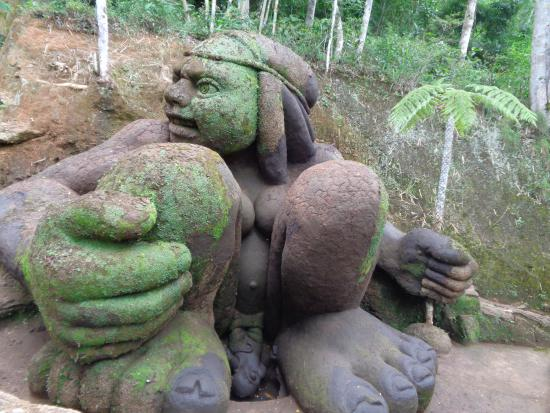
\includegraphics[width=0.45\linewidth]{figs/jardim-do-nego.jpg}
		\quad 
		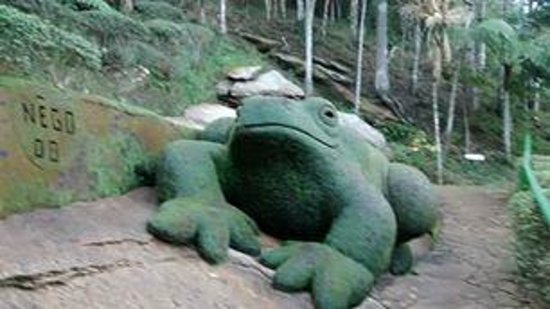
\includegraphics[width=0.5\linewidth]{figs/jardim-do-nego32.jpg}
		\caption{%
			Algumas esculturas criadas por Nêgo 
		}
	\end{figure}
\end{frame}

%\begin{frame} 
%	\begin{figure}[!h]
%		\centering
%		
%	\end{figure}
%\end{frame}
%
%
%\begin{frame} 
%	\begin{figure}[!h]
%		\centering
%		
%	\end{figure}
%\end{frame}

\begin{frame}

Perguntas a serem respondidas ao longo deste projeto:

	\begin{enumerate}
	\item {Que nível de detalhe, facilidade e precisão pode-se obter usando apenas imagens e softwares abertos?}
	\item {É possível utilizar scanners de baixo custo baseados em Kinect com melhorias significativas em termos de qualidade, conveniência ou tempo de processamento?}
	\item {Quais são as restrições desses sitemas?}
	\end{enumerate}
	
\end{frame}

% ---------------------------------------------------------------------------- %
\section{Reconstrução a laser}
% ---------------------------------------------------------------------------- %


\begin{frame}
	\begin{figure}
		\begin{center}
		\centering
		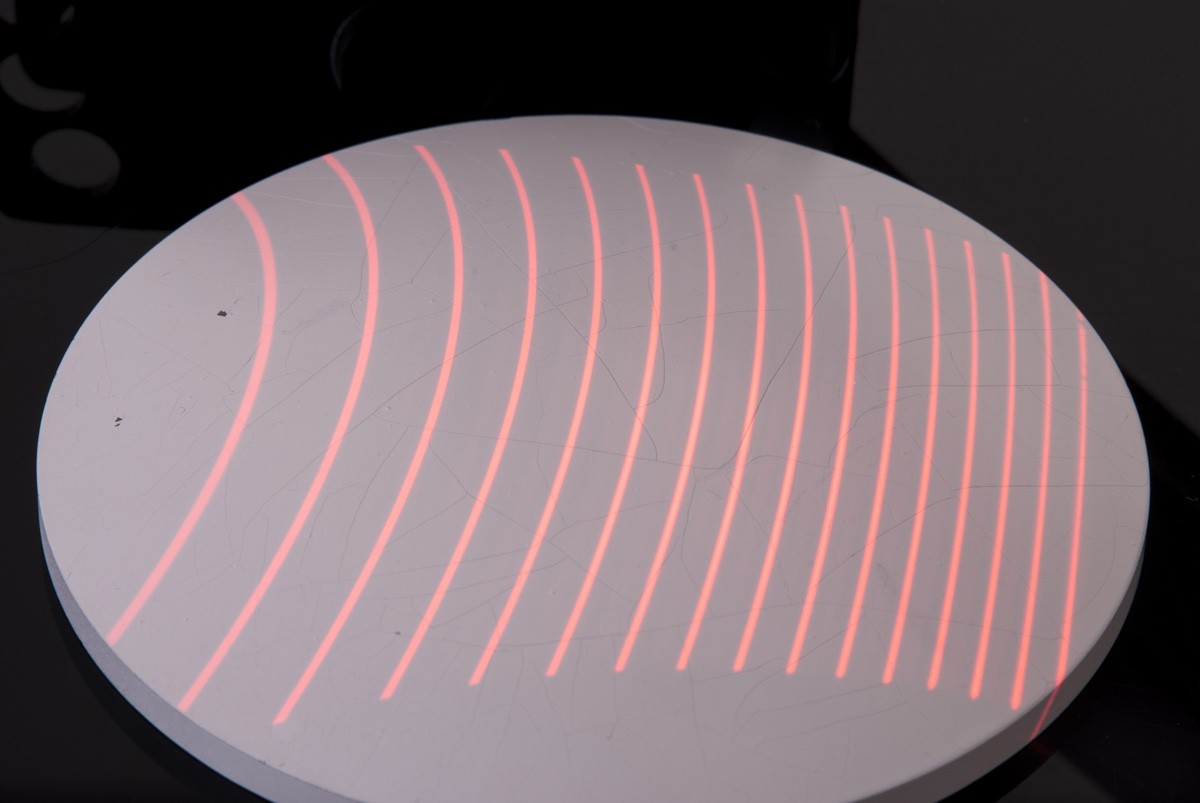
\includegraphics[width=0.7\linewidth]{figs/luzestruturada.jpg}
		\caption{Exemplo de um projetor à laser. \\
		\tiny{Fonte: http://www.opto-engineering.com/}
		}
	\end{center}
\end{figure}	 

\end{frame}

% ---------------------------------------------------------------------------- %
\subsection{Esculturas de Michelangelo}
% ---------------------------------------------------------------------------- %

\begin{frame} 
	\begin{figure}[!h]
		\centering
		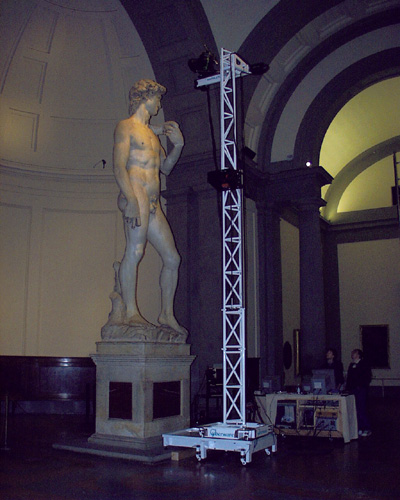
\includegraphics[width=0.4\linewidth]{figs/gantry-and-david4-s.jpg}
		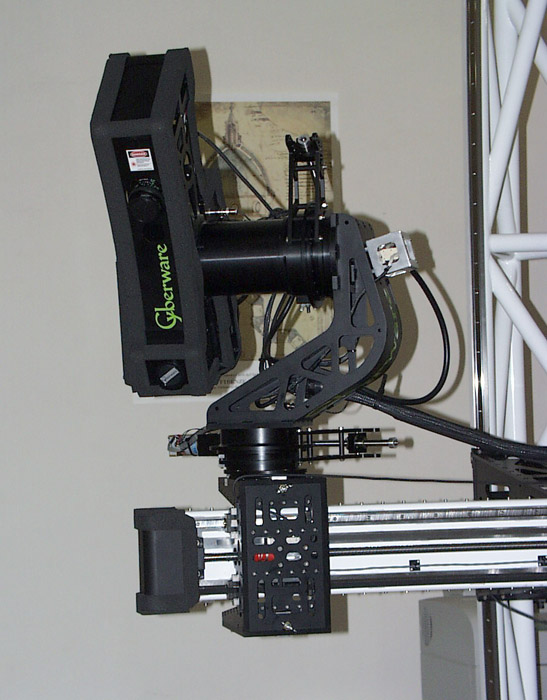
\includegraphics[width=0.4\linewidth]{figs/mgantry-scannerhead-s.jpg}
		\caption{%
		Scanners utilizados no projeto de reconstrução de David. \\
		\tiny{Fonte: http://graphics.stanford.edu/projects/mich/}
		}
	\end{figure}
\end{frame}

\begin{frame} 
	\begin{center}
		\begin{figure}[!h]
			\centering
			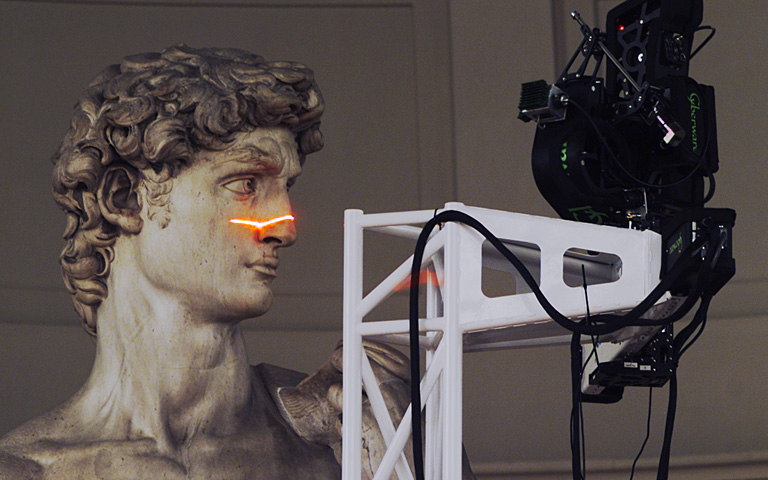
\includegraphics[width=0.7\linewidth]{figs/scanner-head-and-david-head-s.jpg}
			\caption{%
			Exemplo de escaneamento da cabeça de David. \\
			\tiny{Fonte: http://graphics.stanford.edu/projects/mich/}
			}
		\end{figure}
	\end{center}
\end{frame}

\begin{frame} 
	\begin{center}
		\centering
		\begin{figure}[!h]
			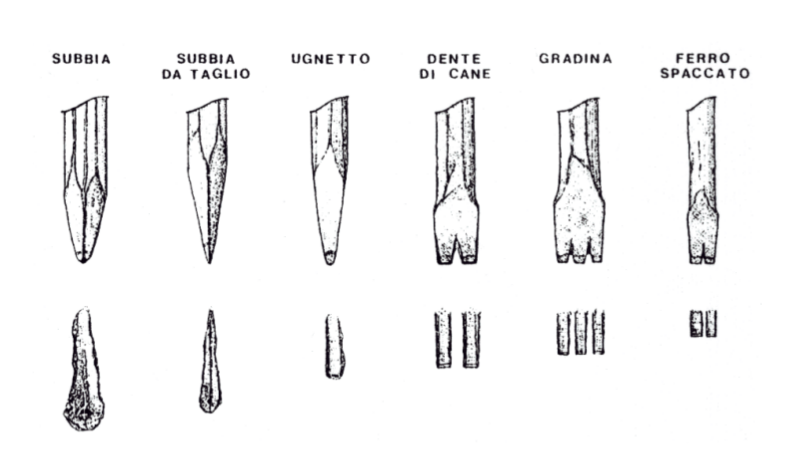
\includegraphics[width=0.7\linewidth]{figs/ferramentasMich.png}
			\caption{%
			Exemplos de cinzéis usados por Michelangelo \\
			\tiny{Fonte: http://graphics.stanford.edu/projects/mich/}
			}
		\end{figure}
	\end{center}
\end{frame}

% ---------------------------------------------------------------------------- %
\section{\protect\emph{Structure from Motion}}
% ---------------------------------------------------------------------------- %

\begin{frame}
	\begin{center}
		\begin{figure}[!h]
			\centering
			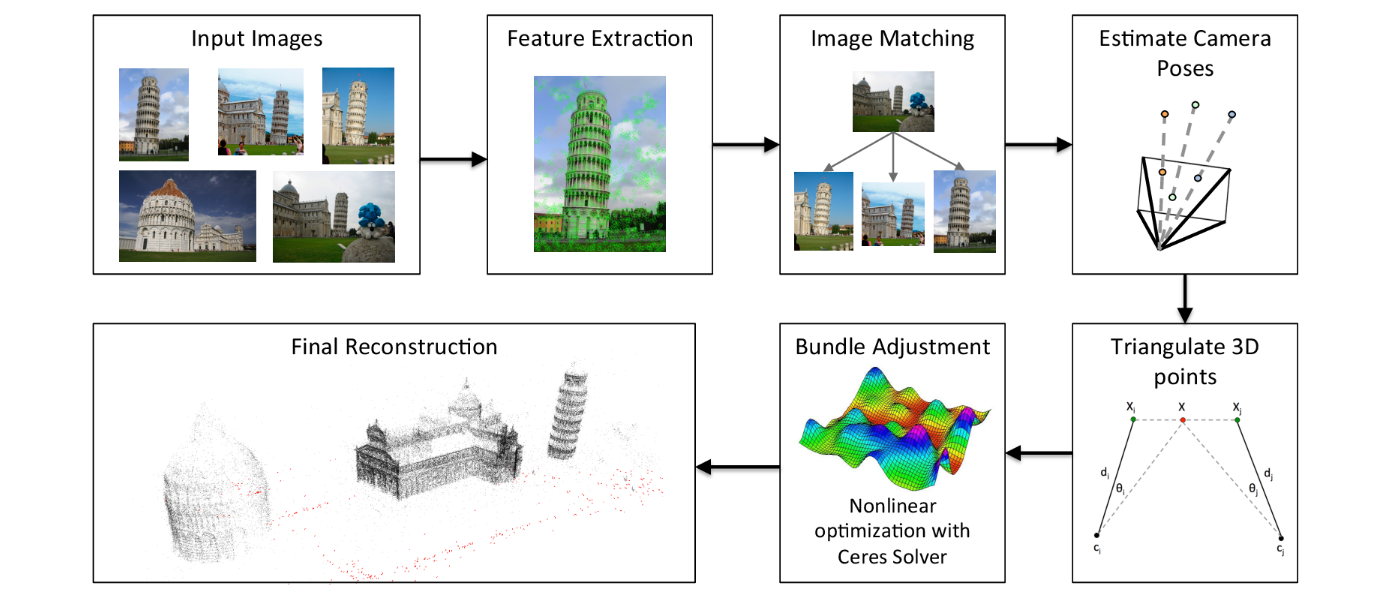
\includegraphics[width=1\linewidth]{figs/pipelinesfm.png}
			\caption{%
				Processo do SfM \\
			\tiny{Fonte: http://www.theia-sfm.org/sfm.html}
			}
		\end{figure}	
	\end{center}
\end{frame}
%
%\begin{frame}
%\frametitle{\textbf{SIFT -- \emph{Scale Invariant Feature Transform}}}
%	\begin{center}		
%		\begin{figure}[!h]
%			\centering
%			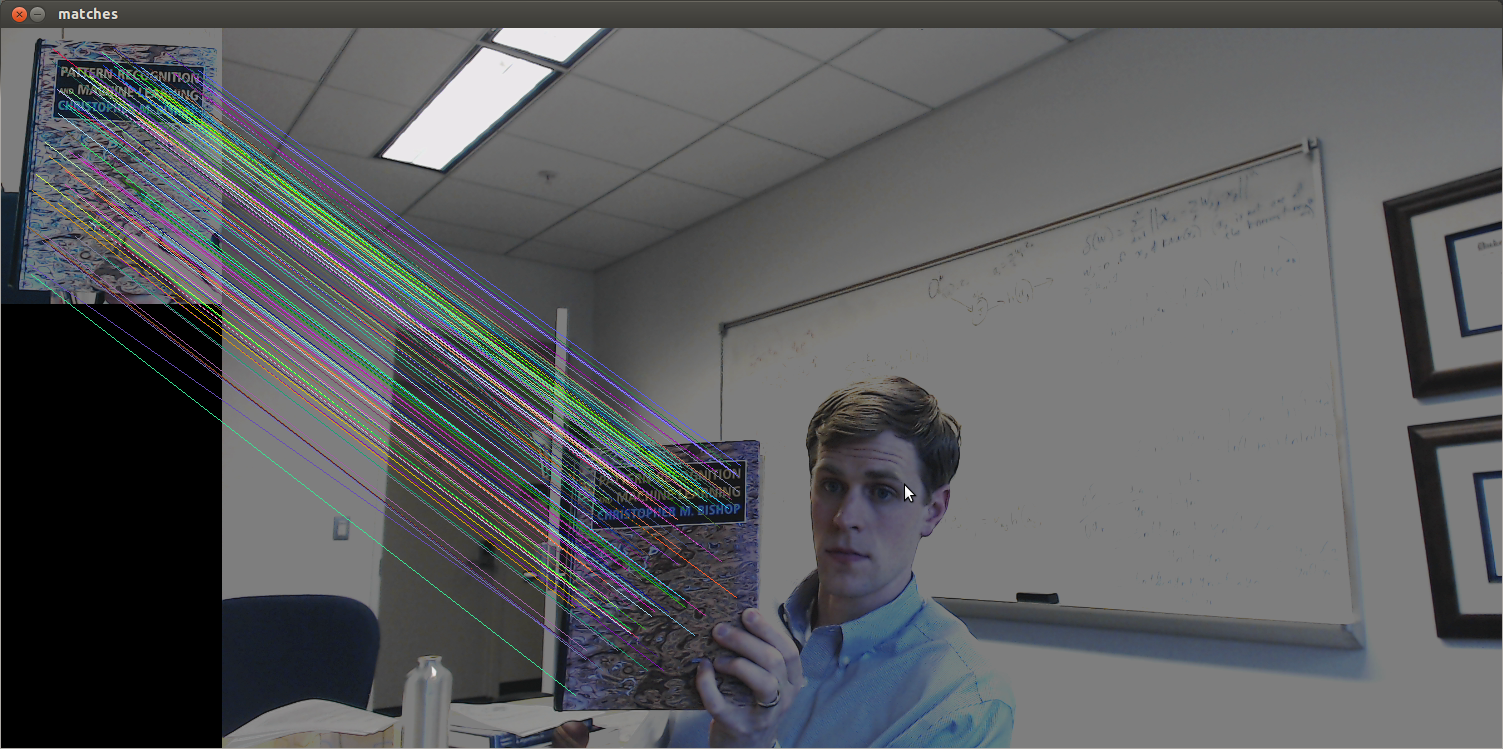
\includegraphics[width=1\linewidth]{figs/sift1.png}
%			\caption{%
%				Exemplo de correspondências SIFT. \\
%			\tiny{Fonte: https://www.usna.edu/Users/cs/taylor/courses/si475/index.php?page=class/siftProject.html}
%			}
%		\end{figure}
%	\end{center}
%\end{frame}

\begin{frame}
\frametitle{\textbf{SIFT -- \emph{Scale Invariant Feature Transform}}}
	\begin{center}		
		\begin{figure}[!h]
			\centering
			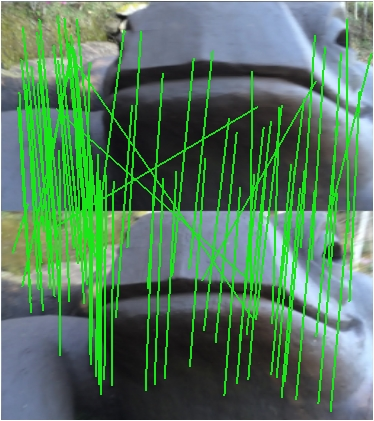
\includegraphics[width=0.5\linewidth]{figs/SIFTsapo.jpg}
			\caption{%
				Exemplo de correspondências SIFT.
			}
		\end{figure}
	\end{center}
\end{frame}

\begin{frame}
\frametitle{\textbf{SIFT -- \emph{Scale Invariant Feature Transform}}}
	\begin{center}		
		COLOCAR IMAGEM DE CORRESPONDENICAS DO INDIO
	\end{center}
\end{frame}


%TODO: COLOCAR IMAGEM DE CORRESPONDENICAS DO INDIO%

\begin{frame}
\frametitle{\textbf{SIFT -- \emph{Scale Invariant Feature Transform}}}
	\begin{center}		
		\begin{figure}[!h]
			\centering
			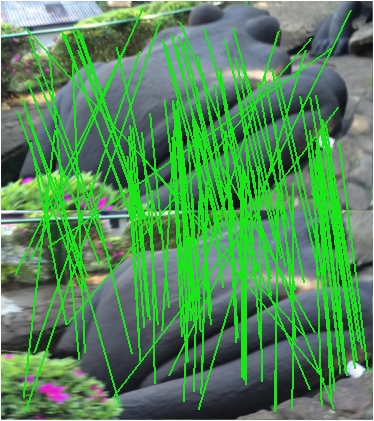
\includegraphics[width=0.5\linewidth]{figs/SIFTsapo2.jpg}
			\caption{%
				Exemplo de correspondências SIFT. \\
			}
		\end{figure}
	\end{center}
\end{frame}

\begin{frame}
\frametitle{\textbf{Triangulação}}
	\begin{center}
		\begin{figure} [!h]
			\centering
			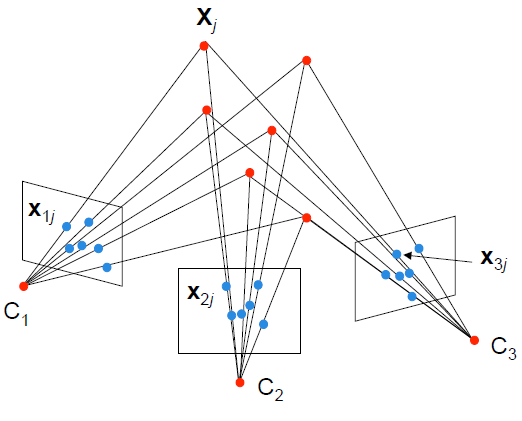
\includegraphics[width=0.45\linewidth]{figs/triangulacao.png}
			\caption{%
				Uma triangulação utilizando um ponto qualquer, $X_j$. Onde cada câmera $C_1, C_2, C_3$ possui um \emph{feature} correspondente a cada uma delas, respectivamente, $X_{1j}, X_{2j}, X_{3j}$. \\
				\tiny{Fonte: http://cs.nyu.edu/~fergus/teaching/vision/11\underline{\space}12\underline{\space}multiview.pdf}
		}
		\end{figure}
	\end{center}
\end{frame}

% ---------------------------------------------------------------------------- %
\subsection{MVE -- \protect\emph{Multi-View Stereo Environment}}
% ---------------------------------------------------------------------------- %

\begin{frame} 
\frametitle{\textbf{MVE -- \emph{Multi-View Stereo Environment}}}
	\begin{center}
		\begin{itemize}
		\item {Reconstrução multi-escala}
		\item {Possui interface gráfica}
		\item {Baseado em mapas de profundidade}
		\item {Implementa um algoritmo de reconstrução de superfícies}
		\end{itemize}
	\end{center}
\end{frame}

\begin{frame}
\frametitle{\textbf{MVE -- \protect\emph{Multi-View Stereo Environment}}}
	\begin{center}
	\begin{figure}
		\centering
		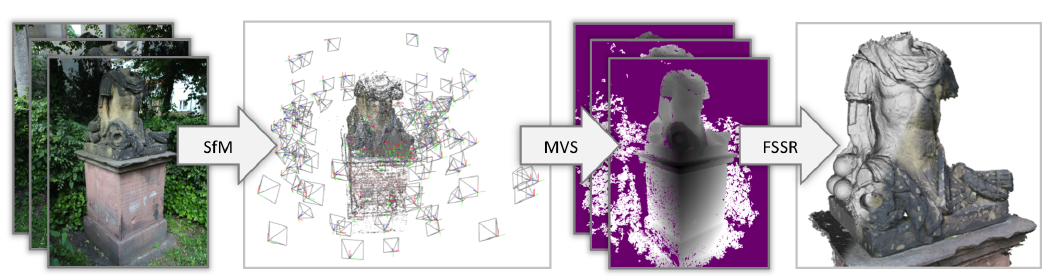
\includegraphics[width=1\linewidth]{figs/mvepipe.png}
	 	\caption{
		Processo empregado pelo MVE. \\
		\tiny{Fonte: https://www.gcc.tu-darmstadt.de/media/gcc/papers/Fuhrmann-2014-MVE.pdf}
	}
	\end{figure}
	\end{center}
\end{frame}

% ---------------------------------------------------------------------------- %
\subsubsection{MVS}
% ---------------------------------------------------------------------------- %

%\begin{frame} 
%\frametitle{\textbf{MVS}}
%	\begin{center}
%		\begin{itemize}
%			\item {Uma estrutura regional-crescente que tem uma fila de candidatos correspondentes, Q, ordenada pelas localizações dos pixels na câmera acrescido de seus valores para profundidade e normais;}
%	\item {Um sistema de correspondências que leva um candidato correspondente como entrada e calcula profundidade, normal e uma confiança de correspondência usando vistas vizinhas fornecidas pela seleção de exibição local.}
%		\end{itemize}
%	\end{center}
%\end{frame}

\begin{frame}
\frametitle{\textbf{MVS}}
	\begin{center}
		\begin{figure}
			\centering
			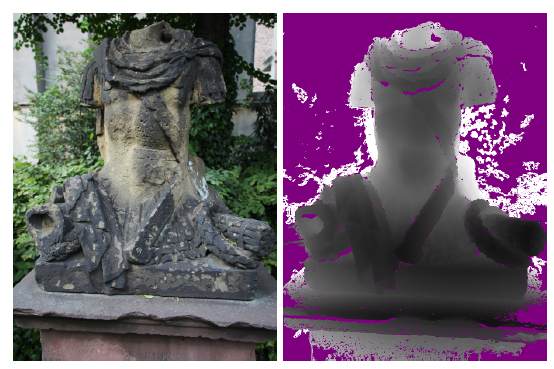
\includegraphics[width=0.8\linewidth]{figs/mvedepth.png}
			\caption{
			Mapa de profundidade de uma imagem. \\
			\tiny{Fonte: https://www.gcc.tu-darmstadt.de/media/gcc/papers/Fuhrmann-2014-MVE.pdf}
			}
		\end{figure}
	 	
	\end{center}
\end{frame}

% ---------------------------------------------------------------------------- %
\subsubsection{FSSR}
% ---------------------------------------------------------------------------- %

\begin{frame}
\frametitle{\textbf{FSSR -- Floating Scale Surface Reconstruction}}
	\begin{center}
	Usa como entrada a união de todos os vértices dos mapas de profundidade. \\
	A partir desses parâmetros ele calcula a representação volumétrica do passo anterior (MVS).
	\end{center}
\end{frame}

\begin{frame}
VER IMAGENS FSSR OU ALGO DO TIPO
\end{frame}
%\begin{frame}
%\frametitle{\textbf{FSSR -- Floating Scale Surface Reconstruction}}
%	\begin{center}
%		\begin{itemize}
%			\item {Utliza uma função implícita e com escala contínua (flutuante);}
%			\item {O FSSR não necessita de muitos parâmetros na sua abordagem abordagem;}
%			\item {A função implícita consegue validar rapidamente os parâmetros de entrada;}
%			\item {Escalável e não requer nenhuma operação global (cortes ou resolução de grandes sistemas de equações).}
%		\end{itemize}
%	\end{center}	  
%\end{frame}
%
%• A reconstrução de uma função implícita contínua e assinada
%com escala espacialmente contínua (escala flutuante) usando um simples
%formulação matemática
%• uma abordagem praticamente sem parâmetros que seleciona a escala de reconstrução apropriada e adapta automaticamente o comportamento de interpolação e aproximação dependendo da redundância nos dados,
%• nenhuma agregação dispendiosa de amostras em um passo de pré-processamento para que a função implícita possa, considerando as amostras de entrada, pronta e rapidamente, e
%• um método eficiente e escalável que não requer nenhum
%operações globais (como a aplicação de cortes de gráficos ou a resolução de grandes
%sistemas de equações).

% ---------------------------------------------------------------------------- %
\subsection{VisualSfM}
% ---------------------------------------------------------------------------- %

\begin{frame} 
\frametitle{\textbf{VisualSfM}}
	\begin{center}
		\begin{itemize}
			\item {Palavra-chave: Escalabilidade}
			\item {Possui interface gráfica}
			\item {Utiliza programação paralela em CPU e GPU}
			\item {Bom gerenciamento dos recursos computacionais}
		\end{itemize}
	\end{center}
\end{frame}

% ---------------------------------------------------------------------------- %
\subsubsection{PBA/MCBA}
% ---------------------------------------------------------------------------- %
\begin{frame} 
\frametitle{\textbf{PBA/MCBA}}
	\begin{center}
		\begin{figure}
			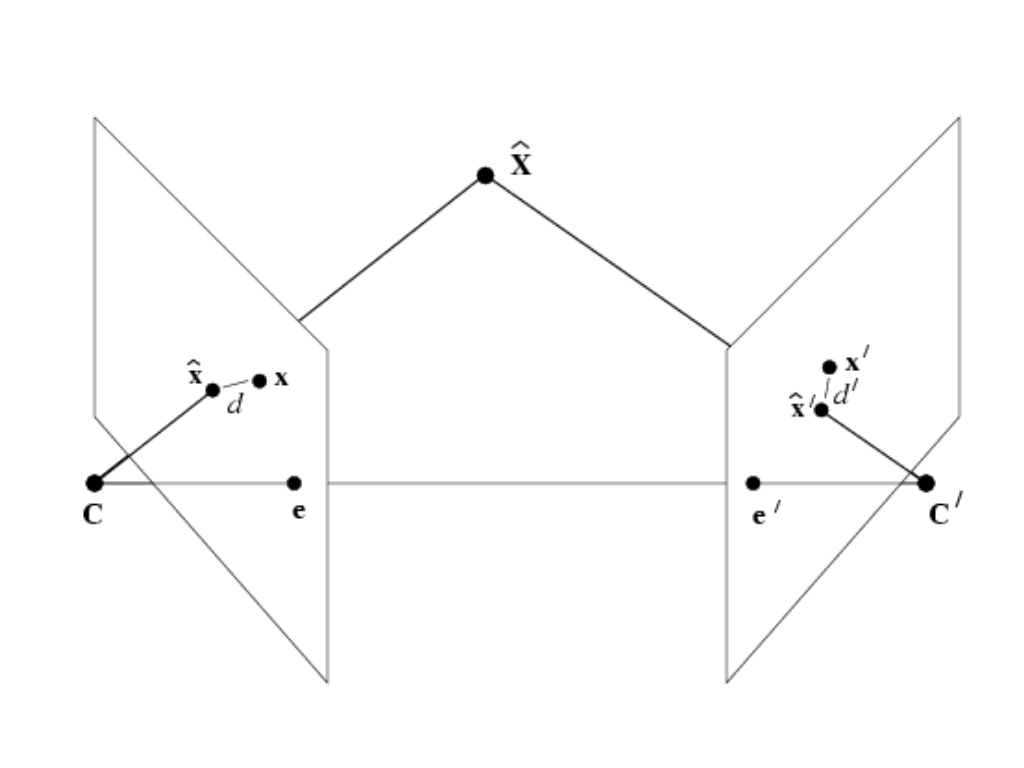
\includegraphics[width=0.6\linewidth]{figs/bundleAdjustment.png}
			\caption{Exemplo do problema de \protect\emph{Bundle Adjustment}. \\
			\tiny{Fonte: http://av.dfki.de/members/stricker/}
			}
		\end{figure}
	\end{center}
\end{frame}

%\begin{frame} 
%\frametitle{\textbf{PBA/MCBA}}
%	\begin{center}
%		\begin{itemize}
%			\item Utiliza Levenberg Mardquardt na resolução do \protect\emph{Bundle Adjustment}.
%			\item Multi-núcleos
%		\end{itemize}
%	\end{center}
%\end{frame}



% ---------------------------------------------------------------------------- %
\subsubsection{CMVS/PMVS-2}
% ---------------------------------------------------------------------------- %

\begin{frame} 
\frametitle{\textbf{CMVS/PMVS-2}}
	\begin{center}
		\begin{figure}
			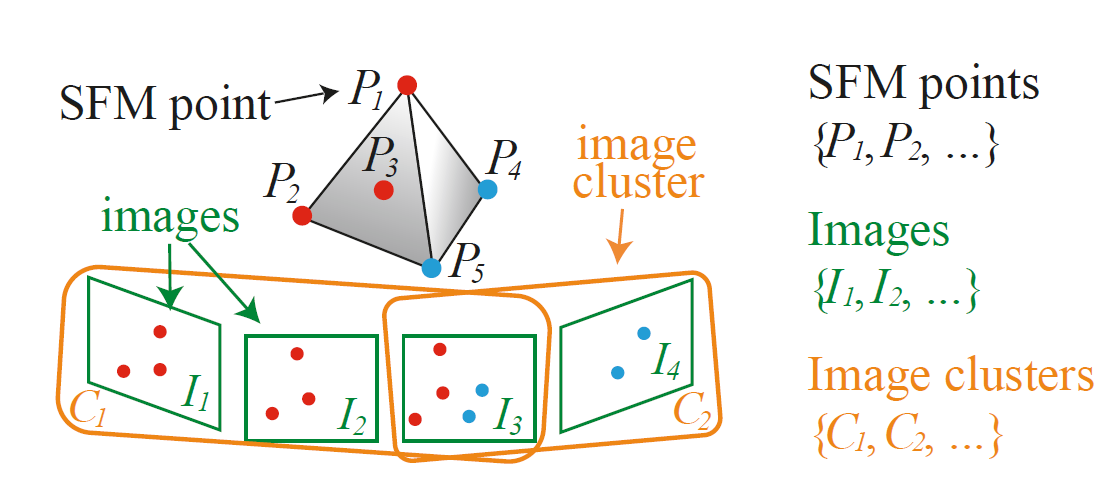
\includegraphics[width=0.8\linewidth]{figs/cmvs.png}
			\caption{Processo do algoritmo CMVS. \\
			\tiny{Fonte: http://ieeexplore.ieee.org/abstract/document/5539802/}
			}
		\end{figure}
	\end{center}
\end{frame}

\begin{frame} 
\frametitle{\textbf{CMVS/PMVS-2}}
	\begin{center}
		\begin{figure}
			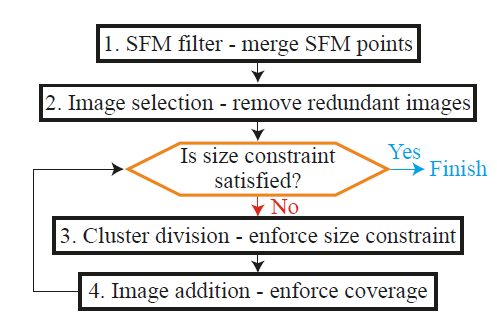
\includegraphics[width=0.7\linewidth]{figs/cmvspipe.png}
			\caption{Processo do algoritmo CMVS. \\
			\tiny{Fonte: http://ieeexplore.ieee.org/abstract/document/5539802/}
			}
		\end{figure}
	\end{center}
\end{frame}


% ---------------------------------------------------------------------------- %
\section{Kinect}
% ---------------------------------------------------------------------------- %
%
%\begin{frame}
%	\begin{itemize}
%		\item {Baseado em luz estruturada}
%		\item {Baseado em \protect\emph{Time of Flight}}
%	\end{itemize}
%\end{frame}

\begin{frame}
	\begin{figure}
		\centering
		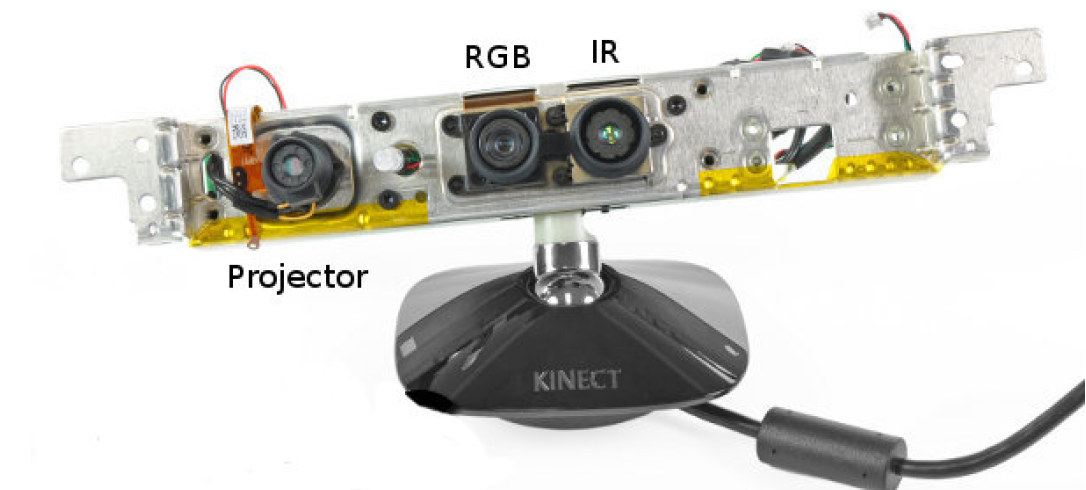
\includegraphics[width=0.5\linewidth]{figs/kinect.png}
		\caption{%
 		 Kinect V1 aberto, constituído de uma câmera infra-vermelho (IR -
 		 \protect\emph{Infra-Red}), uma câmera RGB e um projetor IR.
 		 \tiny{Fonte: http://cmp.felk.cvut.cz/ftp/articles/pajdla/Smisek-CDC4CV-2011.pdf}
		}
	\end{figure}
\end{frame}

\begin{frame}
	\begin{figure}
		\centering
		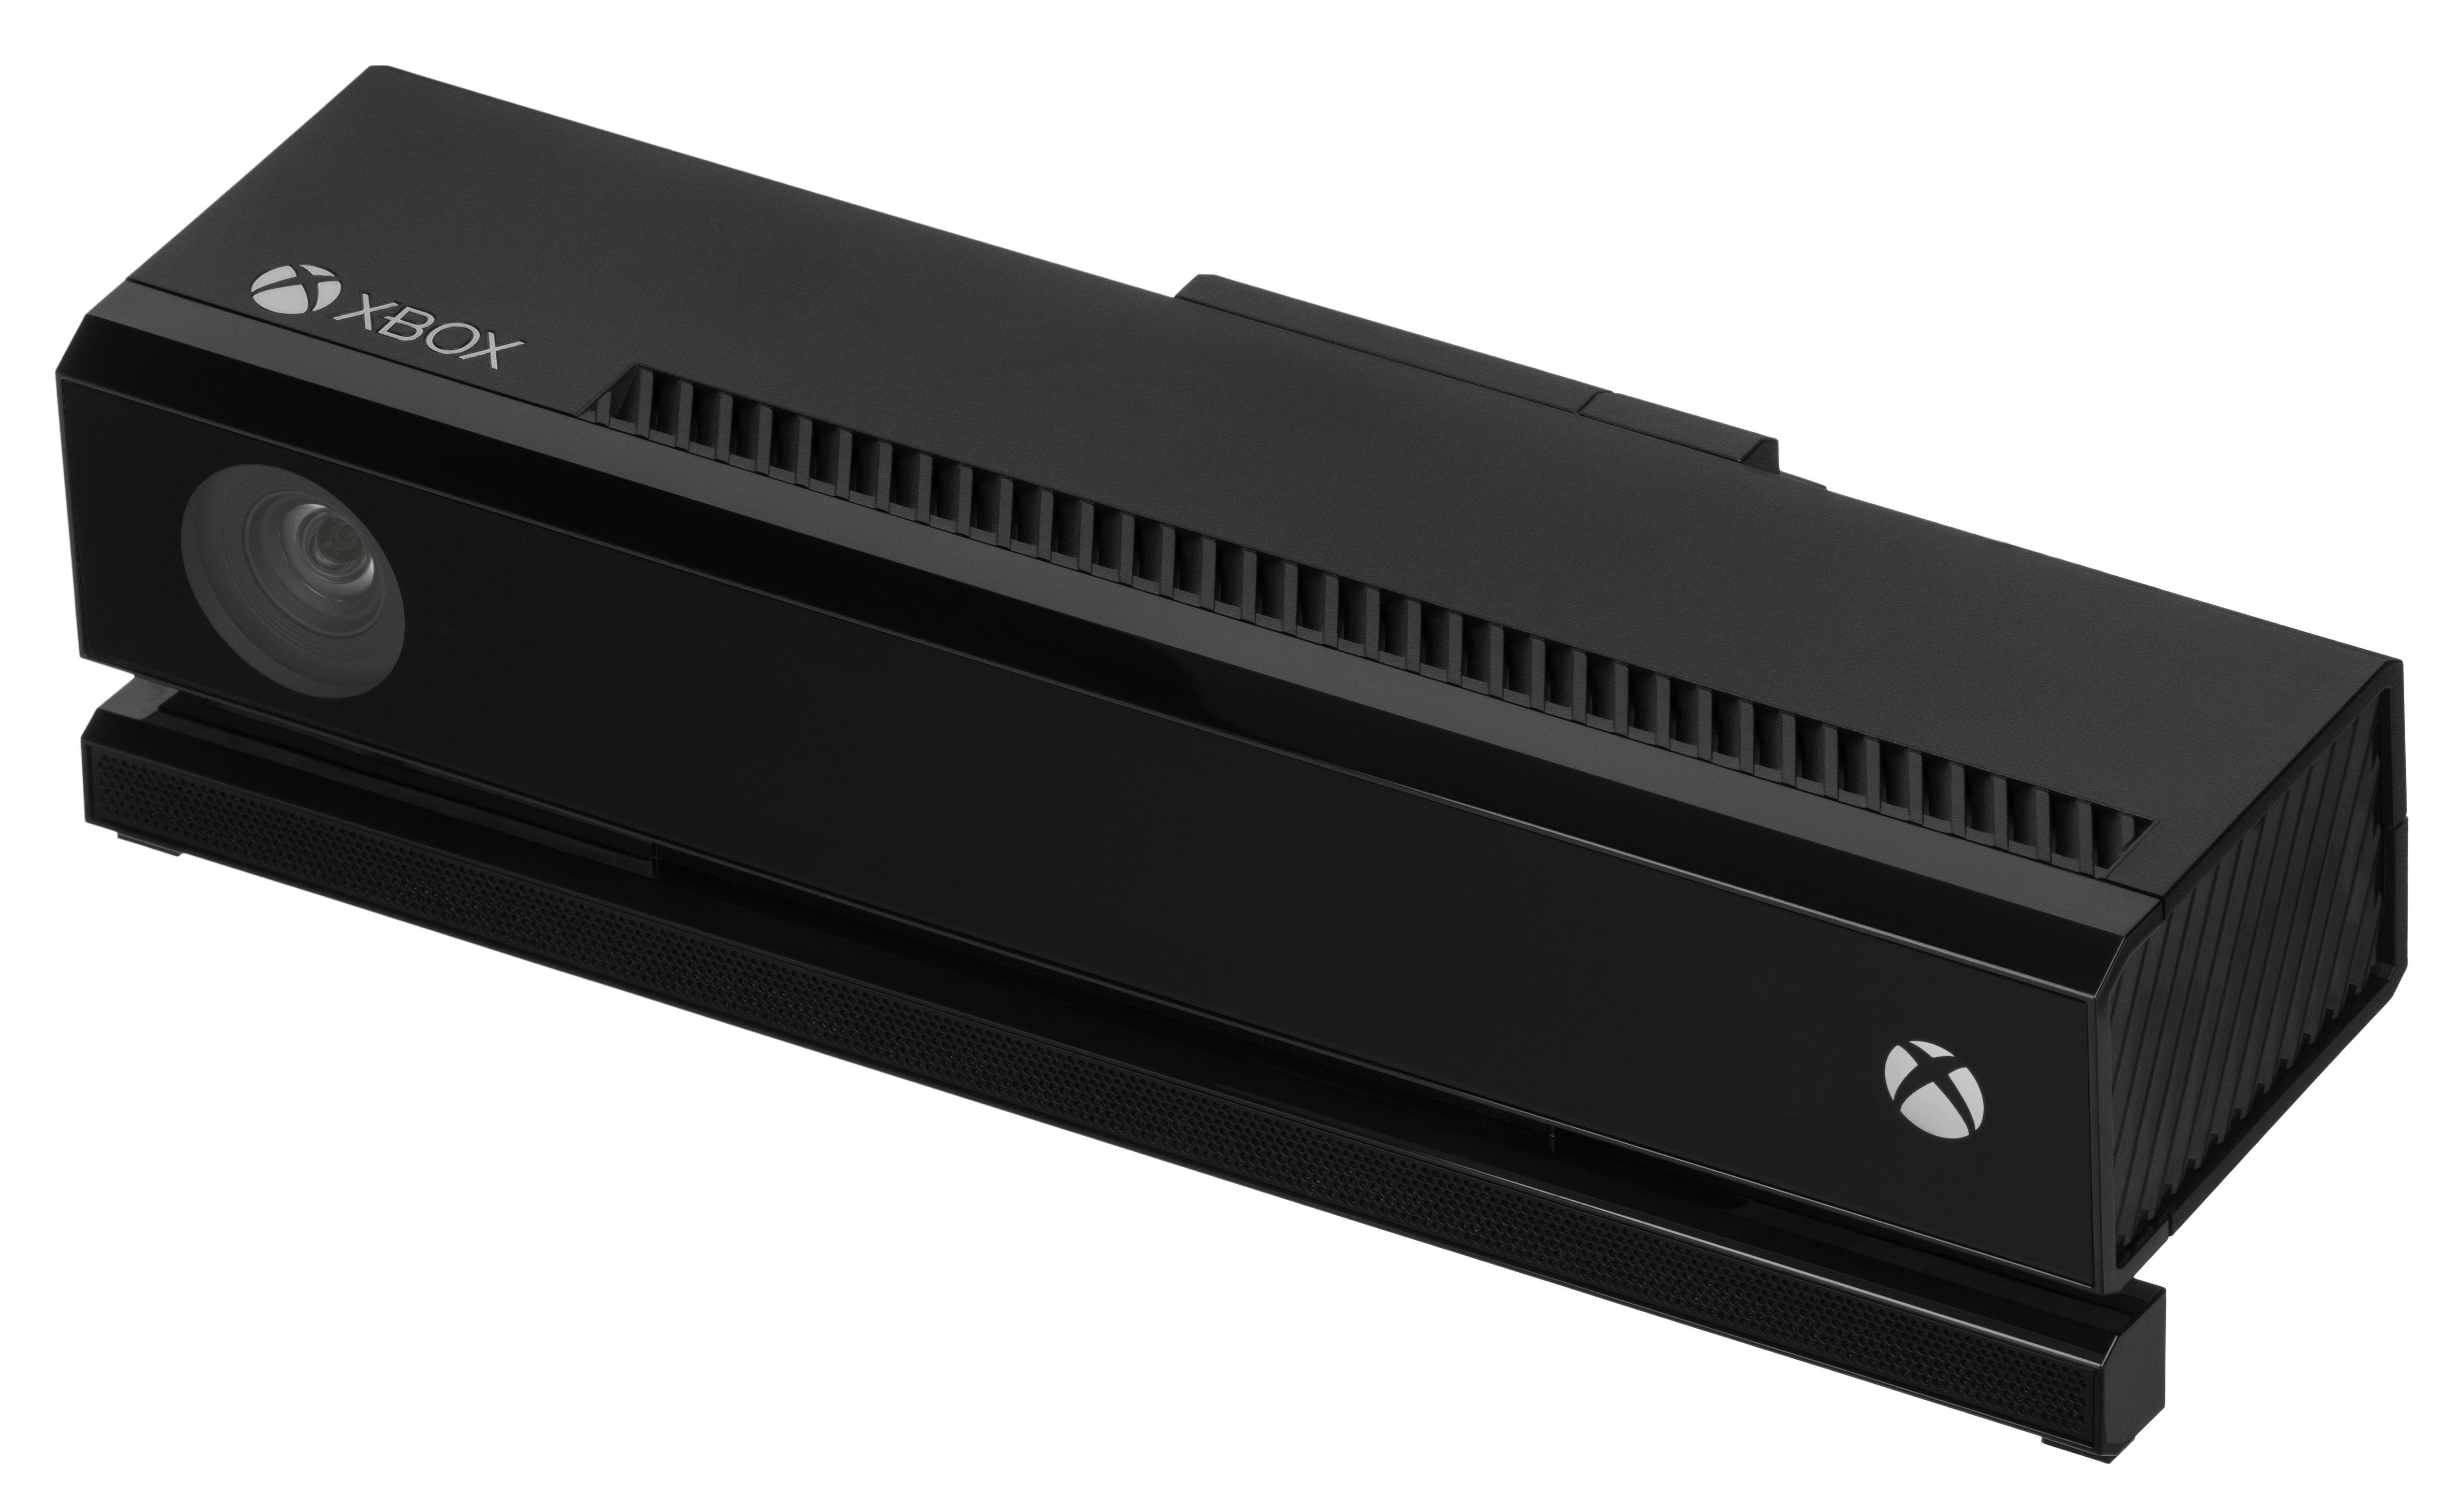
\includegraphics[width=0.5\linewidth]{figs/Xbox-One-Kinect.jpg}
		\caption{%
 		 Kinect V2.
		}
	\end{figure}
\end{frame}

\begin{frame}
	\begin{figure}
		\centering
		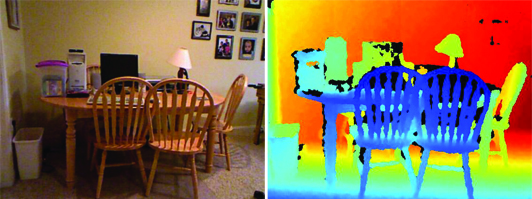
\includegraphics[width=1\linewidth]{figs/profundidadekinect.png}
		\caption{%
 			 Saída de uma imagem interpretada pelo Kinect.
		}
	\end{figure}
\end{frame}

\begin{frame}
	\begin{figure}
		\subfloat[Imagem IR iluminada pelo projetor de padrões IR]{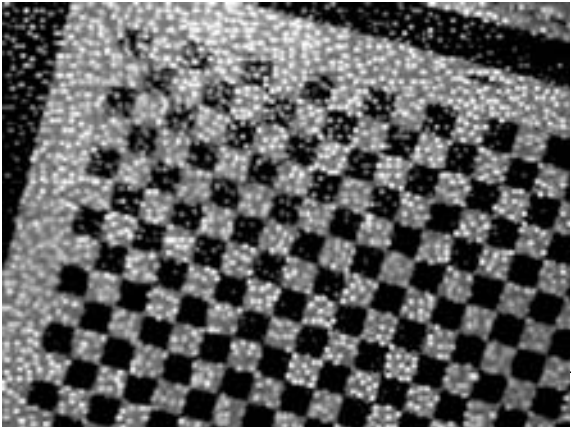
\includegraphics[width=0.2\linewidth]{figs/kinect1.png}}
		\subfloat[Imagem IR com iluminação externa]{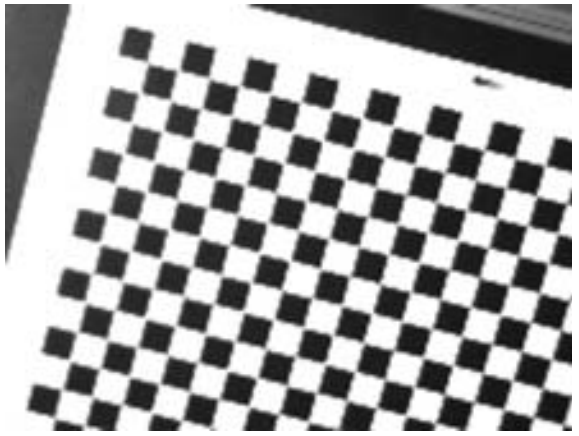
\includegraphics[width=0.2\linewidth]{figs/kinect2.png}}
		\subfloat[Pontos de calibração reproduzidos na imagem RGB]{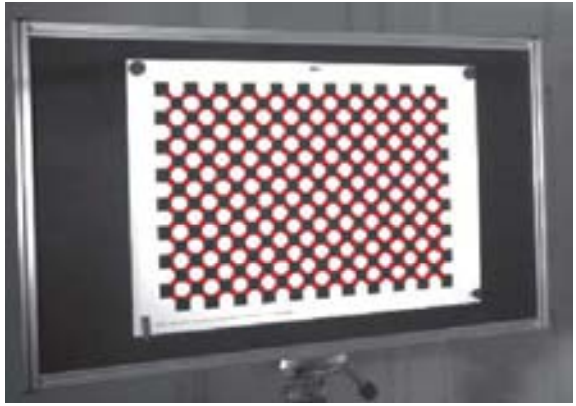
\includegraphics[width=0.2\linewidth]{figs/kinect3.png}}
		\subfloat[Pontos de calibração reproduzidos na imagem de profundidade]{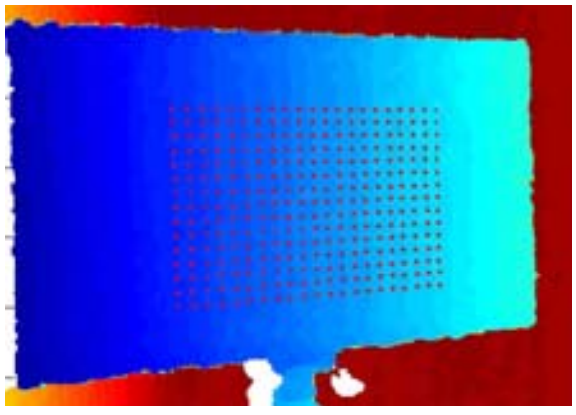
\includegraphics[width=0.2\linewidth]{figs/kinect4.png}}
		\caption{%
		Método de calibração do Kinect, em imagens IR, RGB e de profundidade.
		\tiny{Fonte: http://cmp.felk.cvut.cz/ftp/articles/pajdla/Smisek-CDC4CV-2011.pdf}}
	\end{figure}
\end{frame}

% ---------------------------------------------------------------------------- %
\subsection{Kinect com \protect\emph{Structure from Motion}}
% ---------------------------------------------------------------------------- %
\begin{frame}
	\begin{center}
		\begin{table}[htbp]
\caption{Resultados dos testes executados}
\label{tab:resultadosKinect}
\begin{center}
\begin{tabular}{|c|c|c|c|}
\hline
\multirow{2}{1.5cm}{Método}& \multicolumn{3}{p{5cm}|}{Erro geométrico $e$ [mm]} \bigstrut \\
\cline{2-4} & \multicolumn{1}{c|}{$\mu$($e$)} & \multicolumn{1}{c|}{$\sigma$($e$)} & \multicolumn{1}{c|}{max($e$)} \bigstrut \\ \hline
SLR Stereo & 1,57 & 1,15 & 7,38 \bigstrut \\ \hline
Kinect & 2,39 & 1,67 & 8,64 \bigstrut \\ \hline
SR-4000 & 27,62 & 18,20 & 133,85 \bigstrut \\ 
\hline
\end{tabular}
\end{center}
\end{table}
	\end{center}
\end{frame}

\begin{frame} 
	\begin{center}
		\begin{figure}
		\subfloat[Imagem do lado esquerdo da câmera SLR]{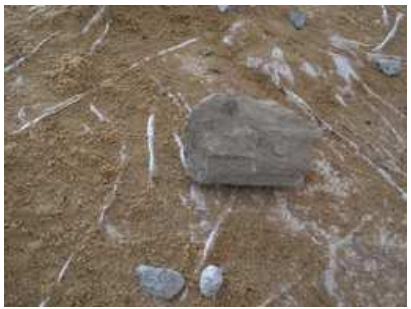
\includegraphics[width=0.3\linewidth]{figs/imagemSLResquerda.png}}
		\subfloat[Imagem da profundidade do Kinect]{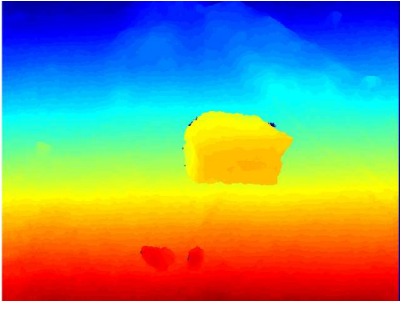
\includegraphics[width=0.3\linewidth]{figs/imagemProfundidadeKinect.png}}
		\subfloat[Imagem do lado direito da câmera SLR]{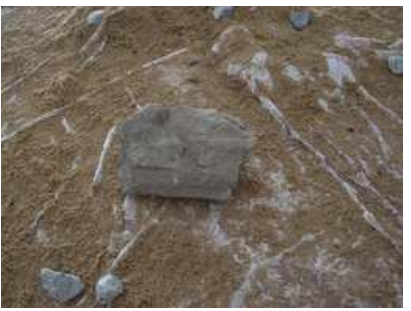
\includegraphics[width=0.3\linewidth]{figs/imagemSLRdireita.png}}
		\caption{%
		Imagens iniciais para reconstrução 3D. \\
		\tiny{Fonte: http://cmp.felk.cvut.cz/ftp/articles/pajdla/Smisek-CDC4CV-2011.pdf}
		}
		\end{figure}
	\end{center}
\end{frame}

\begin{frame}
	\begin{center}
		\begin{figure}
			\centering
			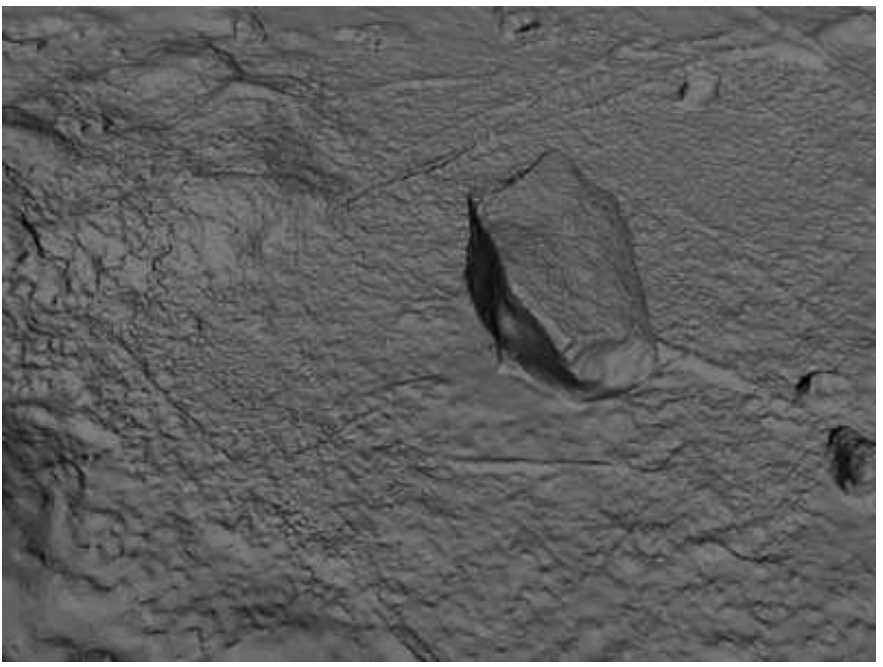
\includegraphics[width=0.3\linewidth]{figs/imagemMVS.png}(a)
			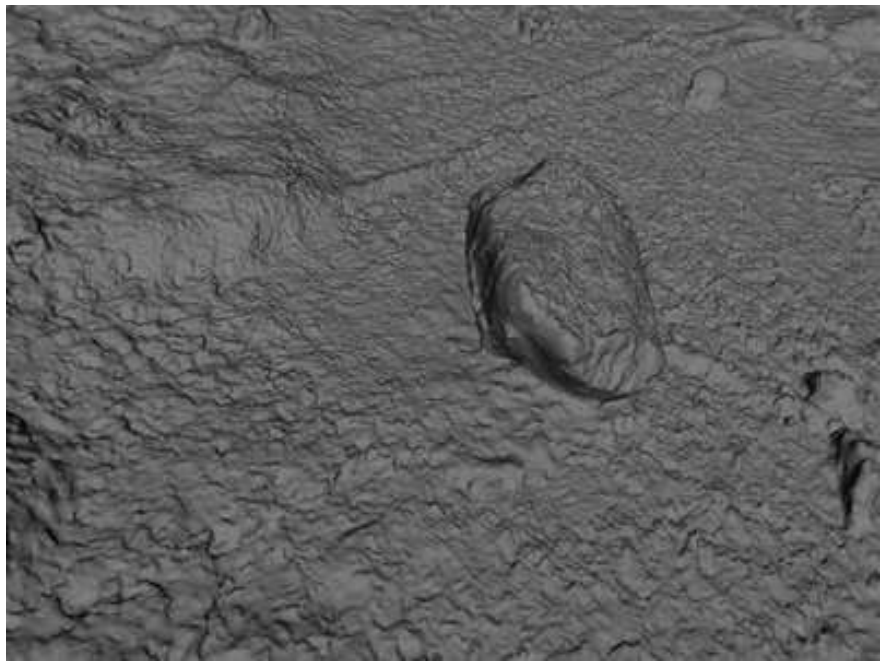
\includegraphics[width=0.3\linewidth]{figs/imagemMVSKinect.png}(b)
			\caption{%
			Resultados da reconstrução SfM, onde (a) é a reconstrução do SLR e (b) o resultado do Kinect. \\
			\tiny{Fonte: http://cmp.felk.cvut.cz/ftp/articles/pajdla/Smisek-CDC4CV-2011.pdf}
			}
			\end{figure}
	\end{center}
\end{frame}

% ---------------------------------------------------------------------------- %
\section{Experimentos}
% ---------------------------------------------------------------------------- %

\begin{frame}
	\begin{figure}
		\centering
		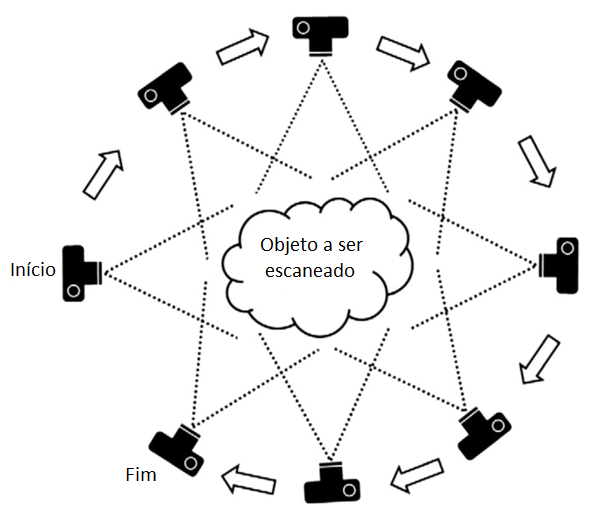
\includegraphics[width=0.7\linewidth]{figs/procedimentoscan.png}
		\caption{%
		Exemplo de como foi realizada a varredura da escultura
		}
	\end{figure}
\end{frame}

\begin{frame}
	Conjuntos de dados:
	\begin{center}
		\begin{itemize}
			\item 2 vídeos em ambiente fechado, com um total de 224 imagens (MVE e VisualSfM);
			\item 2 vídeos de uma escultura (sapo), resultando em 280 imagens (MVE);
			\item 1 vídeo de uma esculutra (índio), resultando em 197 imagens (VisualSfM).
		\end{itemize}
	\end{center}
\end{frame}



% ---------------------------------------------------------------------------- 
\subsection{Objeto em ambiente fechado}
% ---------------------------------------------------------------------------- 

\begin{frame}
	\begin{center}
		\movie[width=160px, height=90px, externalviewer]{Assistir o primeiro video em ambiente fechado}{videos/video1.3gp}
	\end{center}
\end{frame}

\begin{frame}
	\begin{center}
		\movie[width=160px, height=90px, externalviewer]{Assistir o segundo video em ambiente fechado}{videos/video2.3gp}
	\end{center}
\end{frame}

% ---------------------------------------------------------------------------- 
\subsubsection{VisualSfM}
% ---------------------------------------------------------------------------- 

\begin{frame}
\frametitle{\textbf{VisualSfM}}
	\begin{figure}[!h]
		\centering
		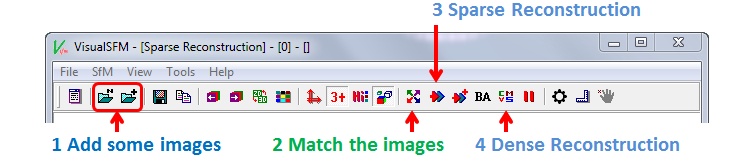
\includegraphics[width=1\linewidth]{figs/pipelinevisualsfm.png}
		\caption{%
		Botões na parte superior da interface gráfica, este seria o procedimento padrão de funcionamento do software. \\
		\tiny{Fonte: http://ccwu.me/vsfm/}
		}
	\end{figure}
\end{frame}

\begin{frame}
\frametitle{\textbf{Objeto com 200 imagens usando o VisualSfM}}
	\begin{table}[h!]
		\caption{Tempos obtidos da reconstrução do objeto com 200 imagens, usando o VisualSfM}
		\begin{tabular}{|l|l|}
			\hline
			Procedimento & Tempo (aprox.) \\ \hline
			Carregamento de imagens & 50 segundos \\ \hline
			Calcular pares correspondentes de \protect\emph{features} & 9.540 segundos \\ \hline
			Gerar a reconstrução esparsa do modelo & 135 segundos \\ \hline
			Gerar a reconstrução densa do modelo & 1.416 segundos \\ \hline
			Total &  11.141 segundos\\ \hline
		\end{tabular}
	\end{table}
\end{frame}

\begin{frame}
\frametitle{\textbf{Objeto com 200 imagens usando o VisualSfM}}
	\begin{figure}[!h]
		\centering
		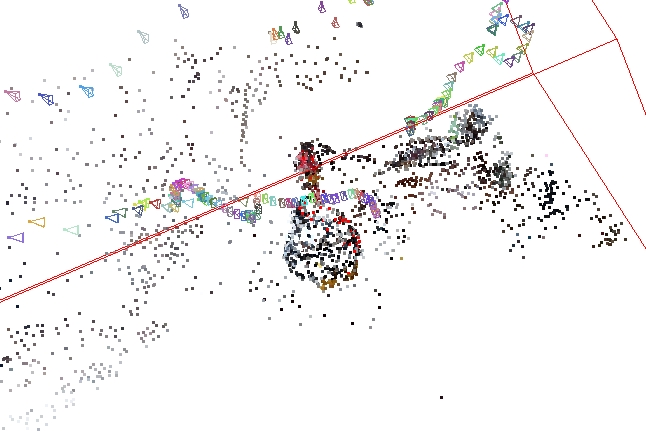
\includegraphics[width=0.8\linewidth]{figs/galinhasparsa.jpg}
		\caption{%
		Reconstrução esparsa do objeto no VisualSfM com 200 imagens.
		}
	\end{figure}
\end{frame}

\begin{frame}
\frametitle{\textbf{Objeto com 200 imagens usando o VisualSfM}}
	\begin{figure}[!h]
		\centering
		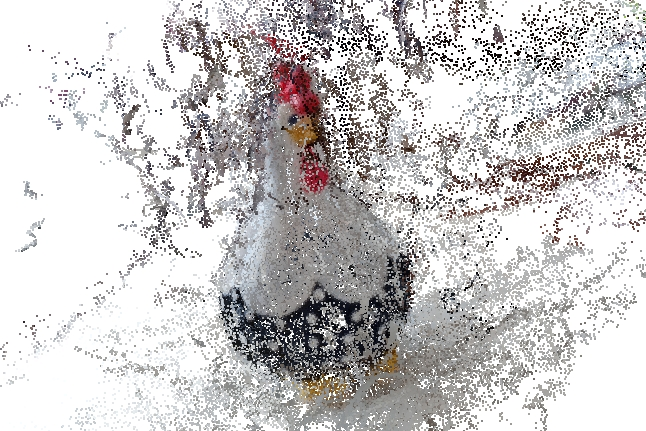
\includegraphics[width=0.8\linewidth]{figs/galinhadense.jpg}
		\caption{%
		Reconstrução densa do objeto no VisualSfM com 200 imagens.
		}
	\end{figure}
\end{frame}

\begin{frame}
\frametitle{\textbf{Objeto com 200 imagens usando o VisualSfM}}
	GALINHA GIRANDO AQUI 200 IMGS!!!
\end{frame}

\begin{frame}
	\frametitle{\textbf{Objeto com 224 imagens usando o VisualSfM}}
	\begin{table}[h!]
		\caption{Tempos obtidos da reconstrução do objeto, com 224 imagens usando o VisualSfM}
		\begin{tabular}{|l|l|}
			\hline
			Procedimento & Tempo (aprox.) \\ \hline
			Carregamento de imagens & 60 segundos \\ \hline
			Calcular pares correspondentes de \protect\emph{features} & 10.451 segundos \\ \hline
			Gerar a reconstrução esparsa do modelo & 162 segundos \\ \hline
			Gerar a reconstrução densa do modelo & 1920 segundos \\ \hline
			Total &  12.593 segundos\\ \hline
		\end{tabular}
	\end{table}
\end{frame}

\begin{frame}
\frametitle{\textbf{Objeto com 224 imagens usando o VisualSfM}}
	\begin{figure}[!h]
		\centering
		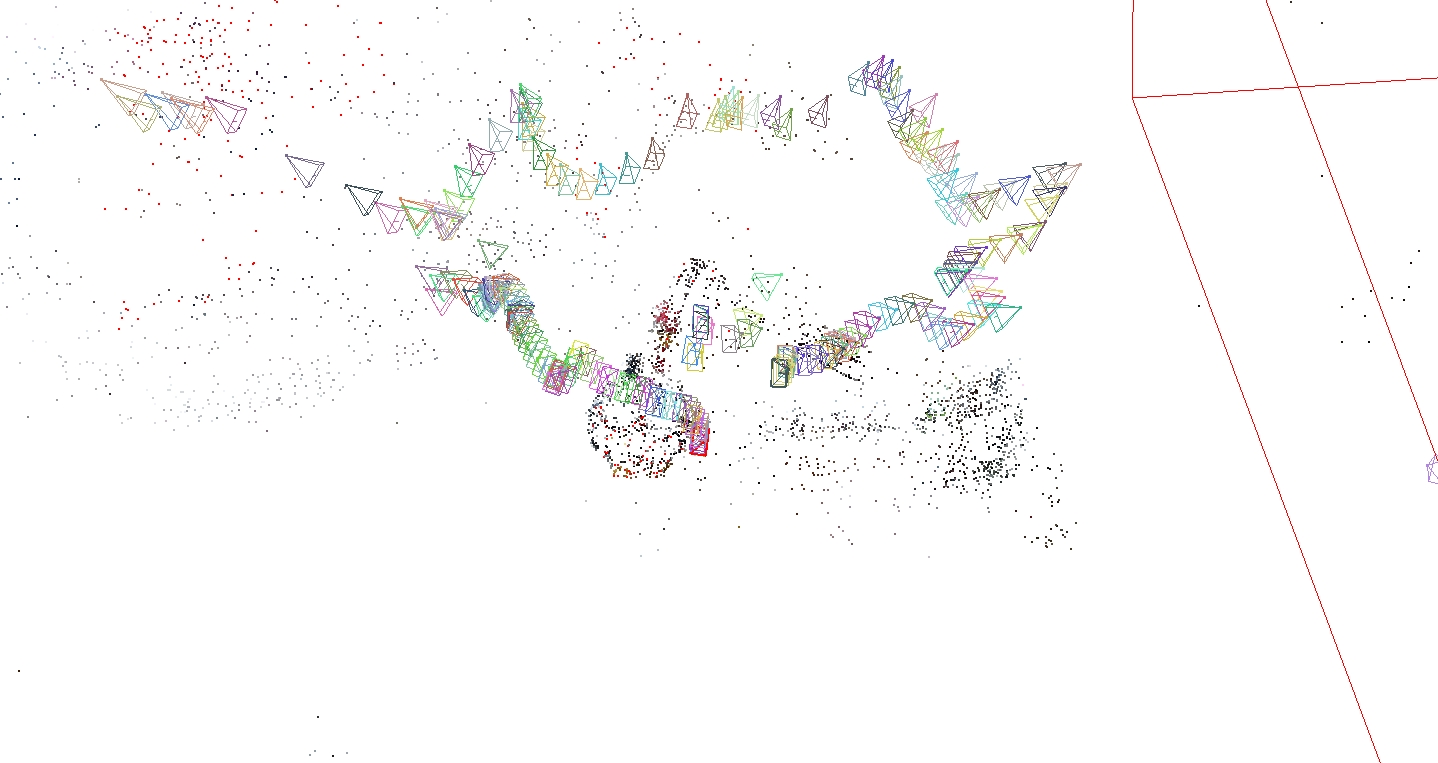
\includegraphics[width=0.7\linewidth]{figs/perto_longe_esparsa.jpg}
		\caption{%
		Reconstrução esparsa do objeto com 224 imagens no VisualSfM.
		}
	\end{figure}
\end{frame}

\begin{frame}
\frametitle{\textbf{Objeto com 224 imagens usando o VisualSfM}}
	\begin{figure}[!h]
		\centering
		\subfloat[]{\label{fig:reconstrucaoDensaVisualSFM2241}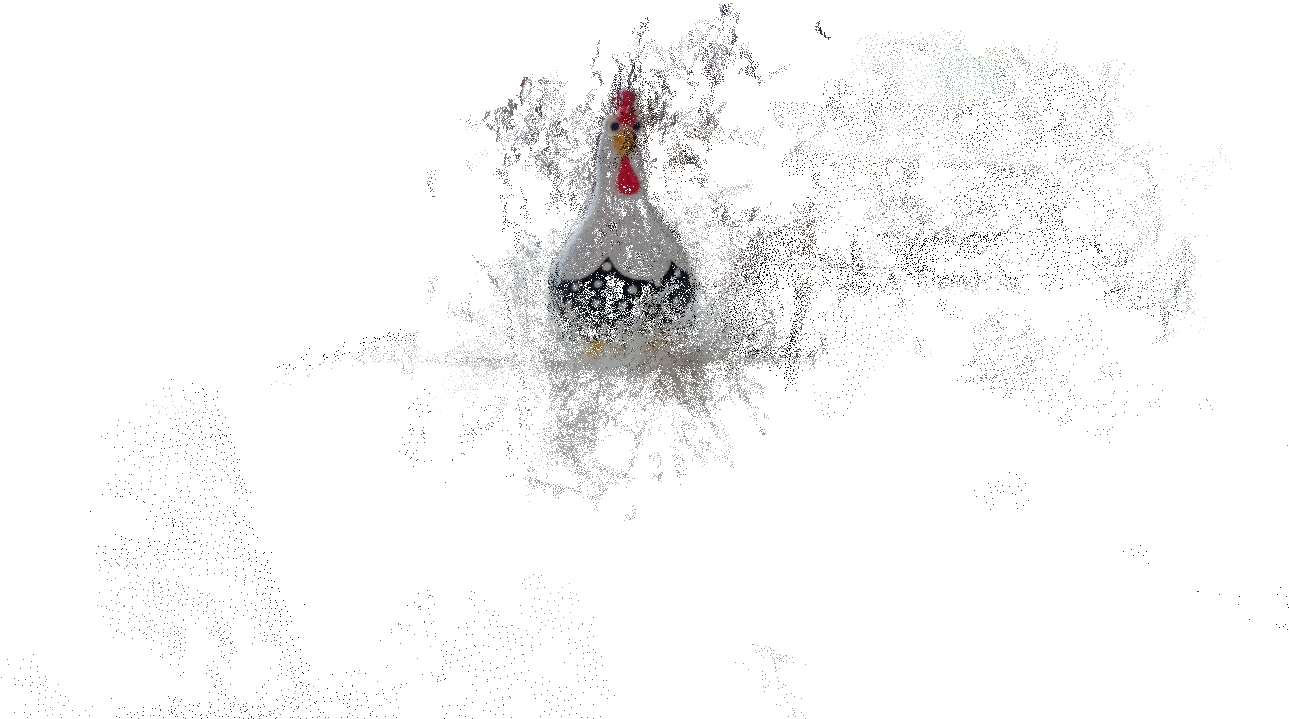
\includegraphics[width=0.45\linewidth]{figs/galinhadense224.jpg}}
		\subfloat[]{\label{fig:reconstrucaoDensaVisualSFM2242}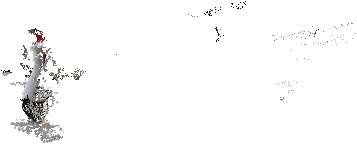
\includegraphics[width=0.45\linewidth]{figs/galinhavisualsfm224.jpg}}
		\caption{Reconstruções densas do primeiro (a) e do segundo (b) modelo do objeto no VisualSfM com 224 imagens.
		}
	\end{figure}
\end{frame}

\begin{frame}
\frametitle{\textbf{Objeto com 224 imagens usando o VisualSfM}}
	GALINHA GIRANDO AQUI 224 IMGS!!!
\end{frame}
% ---------------------------------------------------------------------------- 
\subsubsection{MVE}
% ---------------------------------------------------------------------------- 

\begin{frame}
\frametitle{\textbf{MVE}}
	\begin{figure}[!h]
		\centering
		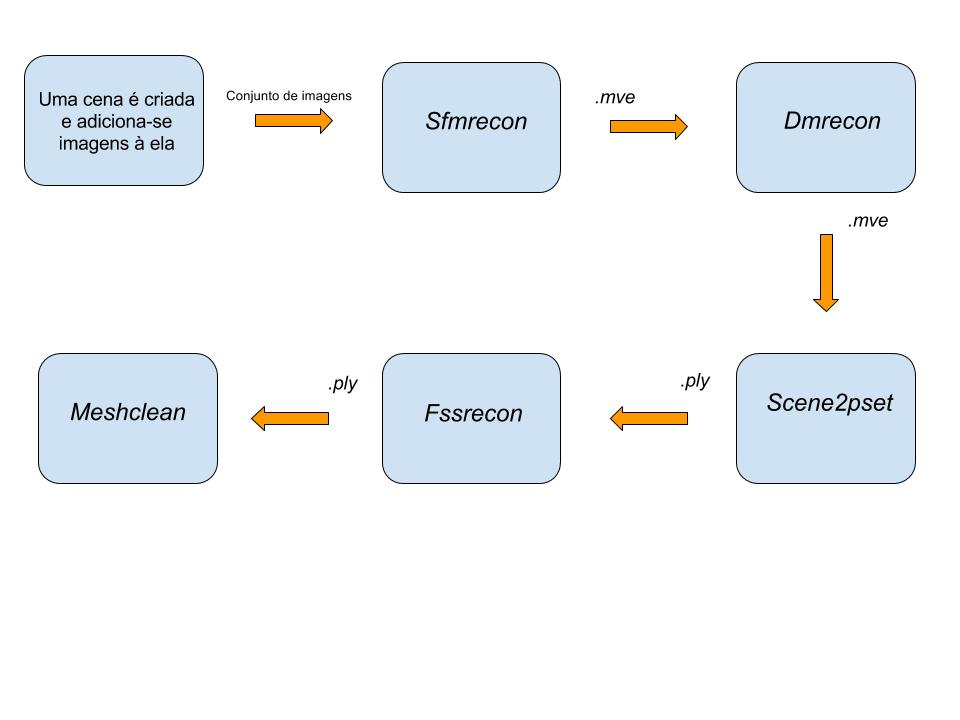
\includegraphics[width=1\linewidth]{figs/pipelineMVE.jpg}
		\caption{%
			Processos no software MVE.
		}
	\end{figure}
\end{frame}

\begin{frame}
\frametitle{\textbf{Objeto com 200 imagens usando o MVE}}
	\begin{table}[!h]
	\centering
	\caption{Tempos obtidos usando o MVE em um conjunto de dados em ambiente interno com 200 imagens}
	\label{tab:galinha200mve}
		\begin{tabular}{|l|l|}
			\hline
			Comando            & Tempo (aprox.)         \\ \hline
			\protect\emph{sfmrecon}  & 371 segundos   \\ \hline
			\protect\emph{dmrecon}   & 3.716 segundos \\ \hline
			\protect\emph{scene2pset} & 300 segundos   \\ \hline
			\protect\emph{fssrecon}  & 1.695 segundos \\ \hline
			\protect\emph{meshclean} & 45 segundos    \\ \hline
			Total & 6.127 segundos \\ \hline
		\end{tabular}
	\end{table}	
\end{frame}

\begin{frame}
\frametitle{\textbf{Objeto com 200 imagens usando o MVE}}
	\begin{figure}[!h]
		\centering
		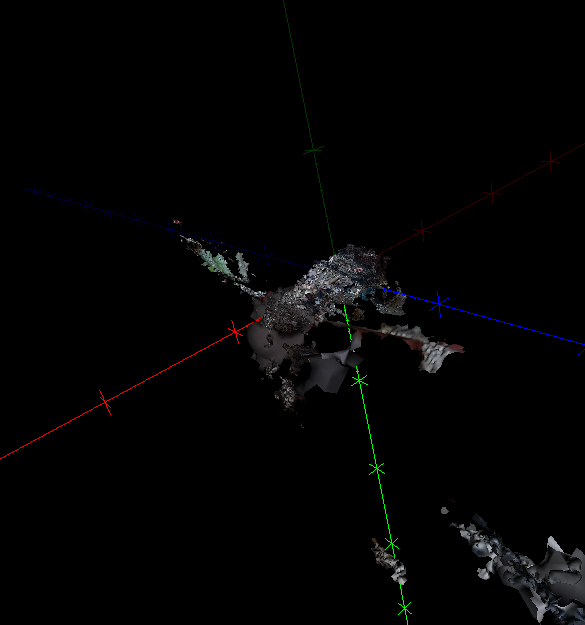
\includegraphics[width=0.5\linewidth]{figs/galinhadmr.png}
		\caption{%
		Resultado da etapa \protect\emph{fssrecon} do MVE
		}\label{fig:galinhaFssr}
	\end{figure}
\end{frame}

\begin{frame}
\frametitle{\textbf{Objeto com 200 imagens usando o MVE}}
	\begin{figure}[!h]
		\centering
		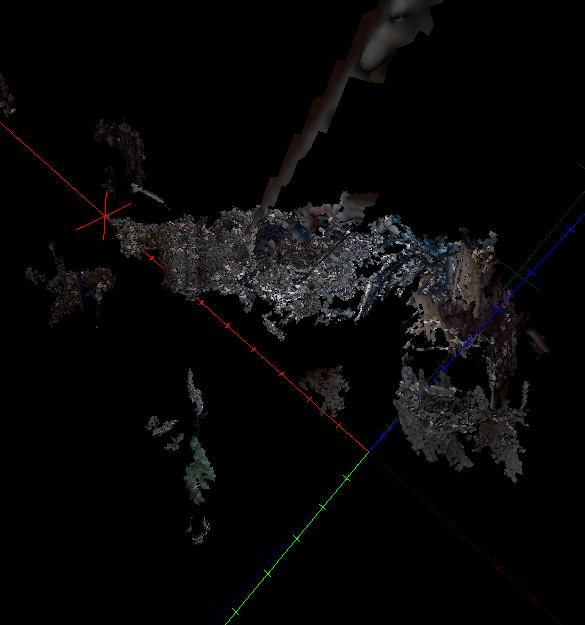
\includegraphics[width=0.5\linewidth]{figs/galinhameshclean.png}
		\caption{%
		Resultado da etapa \protect\emph{meshclean}, da etapa anterior \ref{fig:galinhaFssr}.
		}
	\end{figure}
\end{frame}

\begin{frame}
\frametitle{\textbf{Objeto com 200 imagens usando o MVE}}
	GALINHA GIRANDO AQUI 200 IMGS MVE!!!
\end{frame}

\begin{frame}
\frametitle{\textbf{Objeto com 224 imagens usando o MVE}}
	\begin{figure}[!h]
		\centering
		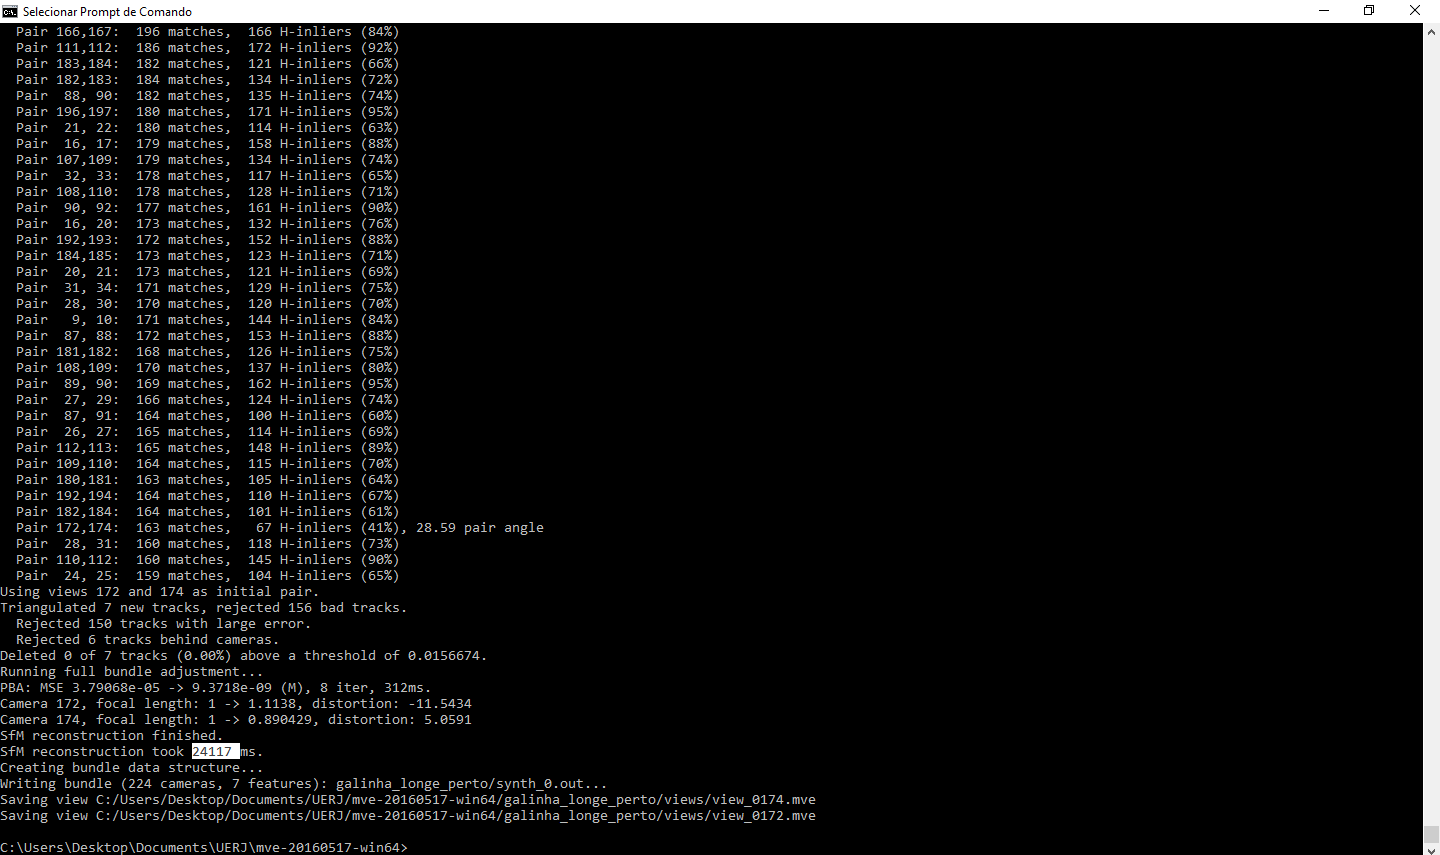
\includegraphics[width=0.8\linewidth]{figs/mvesfmrecongalinhapertolonge.png}
		\caption{%
		Resultado da etapa \protect\emph{sfmrecon}, com todas as imagens.
		}
	\end{figure}
\end{frame}

\begin{frame}
\frametitle{\textbf{Objeto com 224 imagens usando o MVE}}
	\begin{figure}[!h]
			\centering
			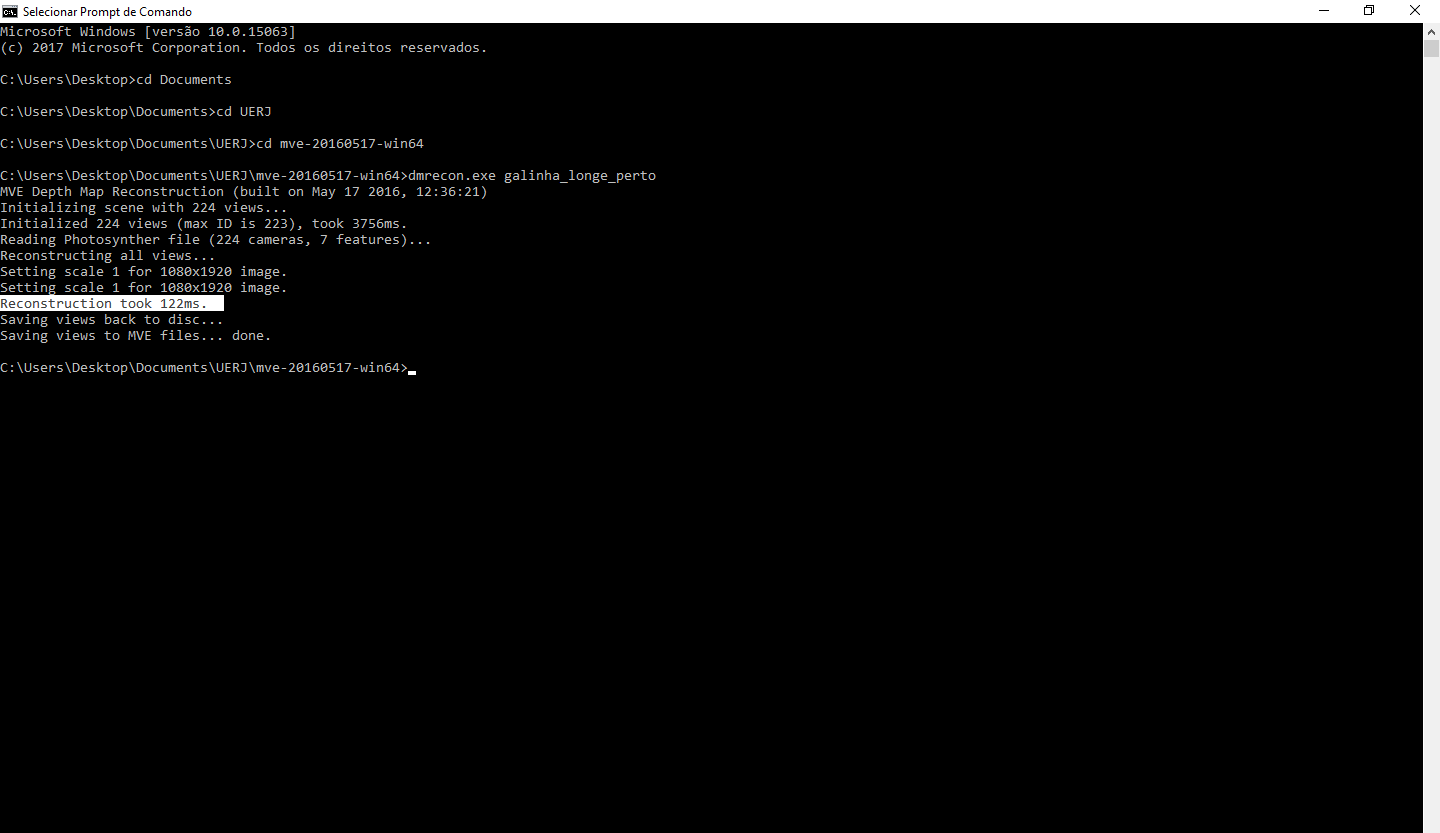
\includegraphics[width=0.8\linewidth]{figs/mvedmrecongalinhapertolonge.png}
			\caption{%
			Resultado da etapa \protect\emph{dmrecon}, com todas as imagens.
			}
	\end{figure}
\end{frame}


% ---------------------------------------------------------------------------- %
\subsection{Escultura do Jardim do Nêgo}
% ---------------------------------------------------------------------------- 

% ---------------------------------------------------------------------------- 
\subsubsection{VisualSfM}
% ---------------------------------------------------------------------------- 

\begin{frame}
\frametitle{\textbf{Escultura com VisualSfM}}
	\begin{center}
		\movie[width=160px, height=90px, externalviewer]{Assistir o video do jardim do Nêgo}{videos/indio.MOV}
	\end{center}
\end{frame}

\begin{frame}
\frametitle{\textbf{Escultura com VisualSfM}}
	\begin{table}
	\caption{Tempos obtidos da reconstrução da escultura do Jardim do Nêgo usando o VisualSfM}
		\begin{tabular}{|l|l|}
			\hline
			Procedimento & Tempo (aprox.) \\ \hline
			Carregamento de imagens & 10 segundos \\ \hline
			Calcular pares correspondentes de \protect\emph{features} & 6.643 segundos \\ \hline
			Gerar a reconstrução esparsa do modelo & 220 segundos \\ \hline
			Gerar a reconstrução densa do modelo & 1.385 segundos \\ \hline
			Total &  8.258 segundos \\ \hline
		\end{tabular}
	\end{table}
\end{frame}

\begin{frame}
\frametitle{\textbf{Escultura com VisualSfM}}
	\begin{figure}[!h]
		\centering
		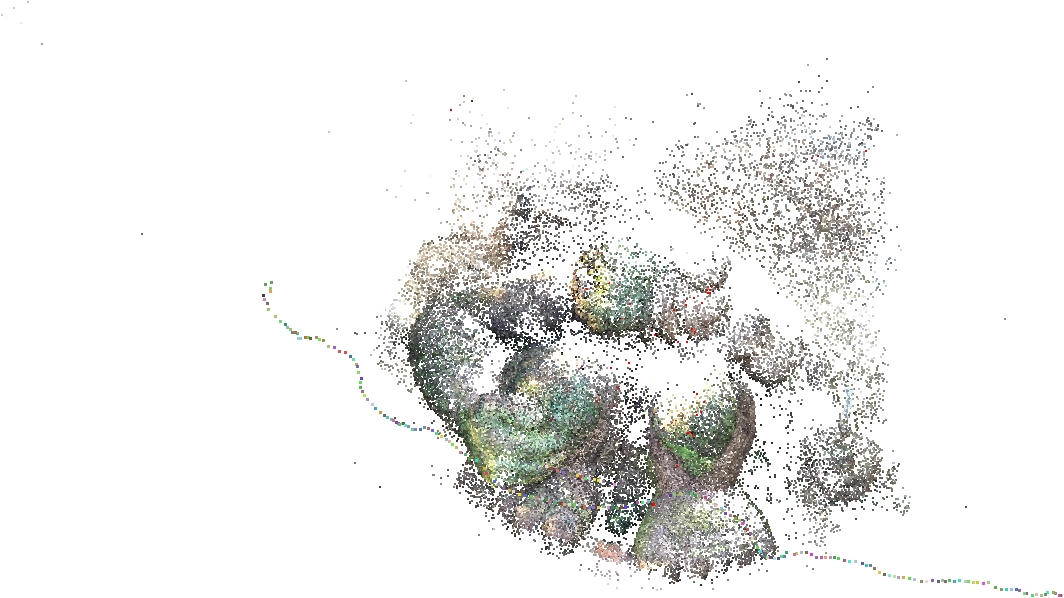
\includegraphics[width=0.9\linewidth]{figs/guerreiroEsparsa.jpg}
		\caption{%
		Reconstrução esparsa da escultura do Jardim do Nêgo no VisualSfM com 197 imagens.
		}\label{fig:reconstrucaoEsparsaIndioVisualSFM}
	\end{figure}
\end{frame}

\begin{frame}
\frametitle{\textbf{Escultura com VisualSfM}}
	\begin{figure}[!h]
		\centering
		\includegraphics[width=0.75\linewidth]{figs/guerreirovisualsfmdmr.jpg}
		\caption{%
		Resultados da reconstrução densa da escultura do Jardim do Nêgo usando o VisualSfM.
		}\label{fig:reconstrucaoDensaIndioVisualSFM}
	\end{figure}
\end{frame}

\begin{frame}
\frametitle{\textbf{Escultura com VisualSfM}}
	\begin{figure}[!h]
		\centering
		\includegraphics[width=0.8\linewidth]{figs/guerreirovisualsfmdmr2.jpg}
		\caption{%
		Resultados da reconstrução densa da escultura do Jardim do Nêgo usando o VisualSfM, em outro ângulo.
		}
	\end{figure}
\end{frame}

\begin{frame}
\frametitle{\textbf{Escultura com VisualSfM}}
	INDIO GIRANDO AQUI!!!
\end{frame}

% ---------------------------------------------------------------------------- 
\subsubsection{MVE}
% ---------------------------------------------------------------------------- 

\begin{frame}
\frametitle{\textbf{Escultura com MVE}}
	\begin{center}
		\movie[width=160px, height=90px, externalviewer]{Assistir o primeiro video do jardim do Nêgo}{videos/sapo1.MOV}
	\end{center}
\end{frame}

\begin{frame}
\frametitle{\textbf{Escultura com MVE}}
	\begin{center}
		\movie[width=160px, height=90px, externalviewer]{Assistir o segundo video do jardim do Nêgo}{videos/sapo2.MOV}
	\end{center}
\end{frame}

\begin{frame}
	\frametitle{\textbf{Escultura com MVE}}
		\begin{figure}[!h]
		\centering
		\includegraphics[width=0.9\linewidth]{figs/umvedense.png}
		\caption{%
		Final da reconstrução via UMVE.
		}\label{fig:UMVEdense}
	\end{figure} 
\end{frame}

\begin{frame}
\frametitle{\textbf{Escultura com MVE}}
	\begin{table}[!h]
	\centering
	\caption{Tempos obtidos usando o MVE em um conjunto de dados do Jardim do Nêgo}
	\label{tab:mveSapo}
		\begin{tabular}{|l|l|}
			\hline
			Comando            & Tempo (aprox.)    \\ \hline
			\protect\emph{sfmrecon}  & 78 segundos     \\ \hline
			\protect\emph{dmrecon}   & 14.503 segundos \\ \hline
			\protect\emph{scene2pset} & 600 segundos    \\ \hline
			\protect\emph{fssrecon}  & 25.293 segundos \\ \hline
			\protect\emph{meshclean} & 60 segundos     \\ \hline
			Total & 40.534 segundos\\ \hline
		\end{tabular}
	\end{table}
\end{frame}

\begin{frame}
\frametitle{\textbf{Escultura com MVE}}
	\begin{figure}[!h]
		\centering
		\includegraphics[width=0.8\linewidth]{figs/mvemeshout.png}
		\caption{%
		Malha com ruídos proveniente do comando \protect\emph{fssrecon}.
		}\label{fig:MVEFSSRMesh}
	\end{figure} 
\end{frame}

\begin{frame}
\frametitle{\textbf{Escultura com MVE}}
	\begin{figure}[!h]
		\centering
		\includegraphics[width=0.8\linewidth]{figs/mvemeshclean.png}
		\caption{%
		Resultado final, após a remoção dos ruídos da malha.
		}\label{fig:MVEMeshClean}
	\end{figure} 
\end{frame}

\begin{frame}
\frametitle{\textbf{Escultura com MVE}}
	SAPO GIRANDO AQUI!!!
\end{frame}


% ---------------------------------------------------------------------------- 
\section{Conclusão}
% ---------------------------------------------------------------------------- 

\begin{frame}
	\begin{center}
	Apresentamos e exploramos técnicas recentes de reconstrução 3D utilizando fotogrametria, relatando problemas e dificuldades encontrados, para justificar a eventual pesquisa em novas técnicas mais avançadas.
	\end{center}
\end{frame}

% ----------------------------------------------------------------------------
\section{Trabalhos futuros}
% ---------------------------------------------------------------------------- 

\begin{frame}
	\begin{enumerate}
    	\item {Realizar uma varredura com o Kinect.}
		\item {Constatar na prática, o melhor método de varredura da escultura.} 
		%\item Automatizar o corte de {\it frames} do vídeo.
		\item {Concretizar o objetivo proposto neste trabalho.}
	\end{enumerate}
\end{frame}

% ---------------------------------------------------------------------------- %
\begin{frame}
	\begin{center}
	{\huge \bf Obrigado! \\
	Perguntas?}
\end{center}
	
\end{frame}


\end{document}

